\hypertarget{simulator}{\section{Simulator}}

\begin{figure}[H]
	\centering
	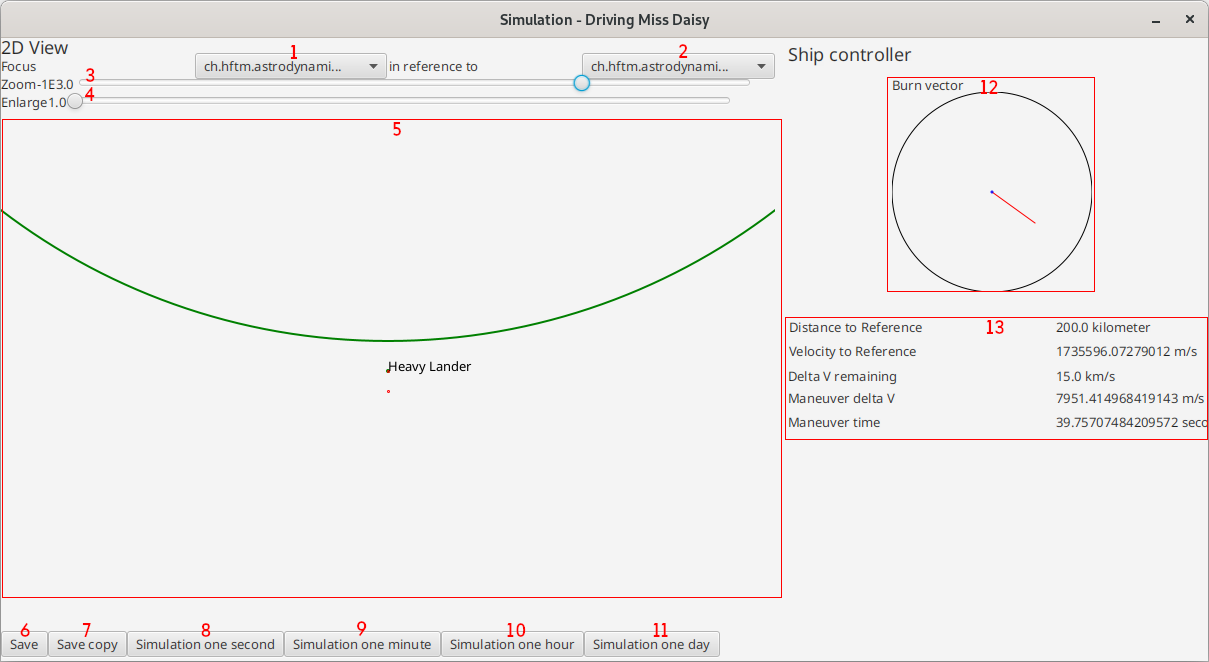
\includegraphics[width=\textwidth]{res/simulation.png}
	\caption[GUI Simulation mit Annotation]{GUI Simulation mit Annotation. Heavy Lander im Fokus, ISS als Referenz}
\end{figure}

\begin{enumerate}[noitemsep]
	\item Fokus-Objekt
	\item Referenz-Objekt
	\item Zoom
	\item Objektvergrösserung
	\item Orbital-View
	\item Save: Speichern der Simulation
	\item Save copy: Kopieren der Simulation
	\item Simulation eine Sekunde berechnen
	\item Simulation eine Minute berechnen
	\item Simulation eine Stunde berechnen
	\item Simulation einen Tag berechnen
	\item Burn vector: Maneuver-Darstellung
	\item Informationspanel
\end{enumerate}

\subsection{Grundlagen}
Der Simulator erlaubt eine simple graphische Darstellung der Simulation. Die linke Seite des Fensters wird dabei von der Orbital-View, auch 2D-View genannt, eingenommen welche ein ortographisches Bild der Objekte darstellt. Mit Zoom und Objektvergrösserung können kleinere und grössere Objekte aufgefunden und zentriert werden. Die rechte Seite des Fensters wird beim Fokus eines Raumschiffs mit der Maneuver-Darstellung welche das geplante Maneuver graphisch darstellt sowie dem Informationspanel gefüllt.

\subparagraph{Objektvergrösserung}
Die Objektvergrösserung skaliert die Darstellung der Objekte in der Orbital-View. Die simulierte Grösse wird dabei nicht verändert. Der Wert \emph{1.0} stellt die Objekte in der Realgrösse dar.

\subparagraph{Maneuver-Vektor}
Der schwarze Kreis stellt die maximal verfügbare Geschwindigkeitsänderung welche das aktuell fokussierte Raumschiff durchführen kann dar. Bei einem aktiven Maneuver wird eine rote Linie in die Richtung in welche die Geschwindigkeitsänderung durchgeführt wird gezogen. Die Linienlänge stellt den benötigten Wert an Geschwindigkeitsänderung gegenüber dem verfügbaren Vorrat (schwarzer Kreis) dar und ändert sich deshalb bei der Durchführung des Maneuvers. Ein Befehl über dem verfügbaren Vorrat ist möglich, es wird jedoch nur bis zum verfügbaren Vorrat durchgeführt.

\subsection{Navigieren im Orbital-View}
Wählen sie das gewünschte Objekt im Fokus-Dropdown aus.
Die Orbital-View fokussiert nun auf das eingestellte Objekt.

\begin{figure}[H]
	\centering
	\begin{minipage}[b]{0.45\textwidth}
		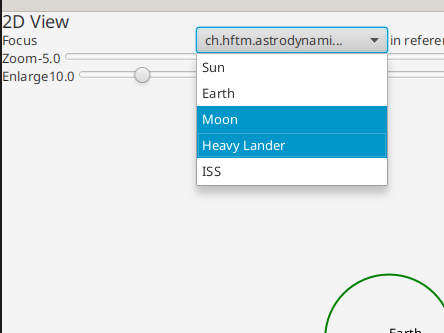
\includegraphics[width=\textwidth]{res/viewfocus.png}
		\caption{Fokus: Ausgangslage Fokus auf Heavy Lander}
	\end{minipage}
	\hfill
	\begin{minipage}[b]{0.45\textwidth}
		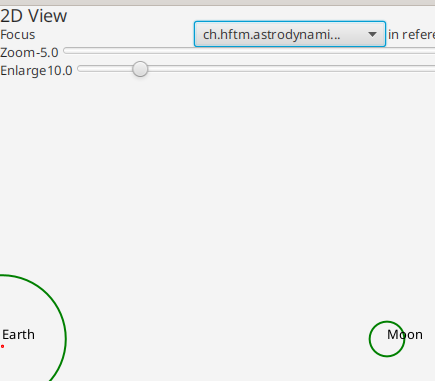
\includegraphics[width=\textwidth]{res/viewfocus2.png}
		\caption{Fokus: Mond zentral im Bild}
	\end{minipage}
\end{figure}

Wählen sie das gewünschte Objekt im Referenz-Dropdown aus.
Informationen über Distanz und Geschwindigkeit relativ zur Referenz werden nun im Informationspanel ausgegeben.
Stellen sie die Zoom-Stufe und eventuelle Objektvergrösserung auf das gewünschte Level ein.
Für Raumschiffe in einem erdnahen Orbit empfielt sich eine Zoomstufe von \emph{-1E3.0} und eine Objektvergrösserungsfaktor von \emph{1.0}.

\subsection{Ausführen eines Maneuvers}
Fokusieren sie ein Raumschiff.
Klicken sie in den schwarzen Kreis der Maneuver-Darstellung.
Eine rote Linie vom Zentrum zu ihrer angeklickten Position erscheint.
Auf dem Informationspanel wird die geplante Geschwindigkeitsänderung (Bezeichnung \emph{Maneuver delta V}) und die Zeitdauer zum Durchführen des Maneuvers (Bezeichnung \emph{Maneuver time}) angegeben.

\begin{figure}[H]
	\centering
	\begin{minipage}[b]{0.45\textwidth}
		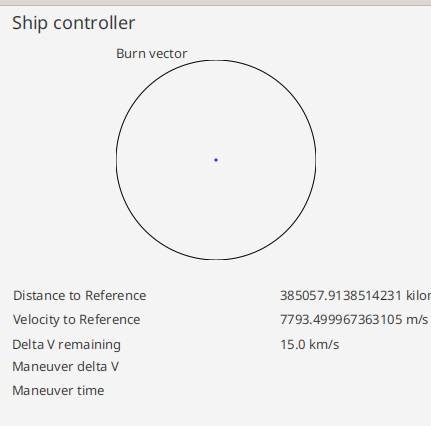
\includegraphics[width=\textwidth]{res/burn1.png}
		\caption{Maneuver: Ausgangslage kein aktives Maneuver}
	\end{minipage}
	\hfill
	\begin{minipage}[b]{0.45\textwidth}
		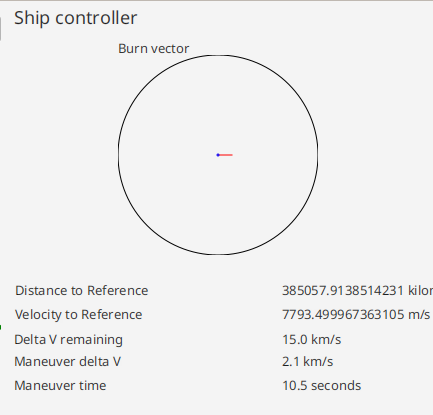
\includegraphics[width=\textwidth]{res/burn2.png}
		\caption{Maneuver: Maneuver aktiv 2.1 km/s delta V in 10.5 sec}
	\end{minipage}
\end{figure}

Klicken sie nun auf einen beliebigen Simulationsbutton bis die Zeitdauer in der Simulation vergangen ist.
Nach ausführen des Maneuvers wird die rote Maneuver-Linie entfernt und die Maneuver-Informationen auf dem Informationspanel ausgeblendet.

\begin{figure}[H]
	\centering
	\begin{minipage}[b]{0.45\textwidth}
		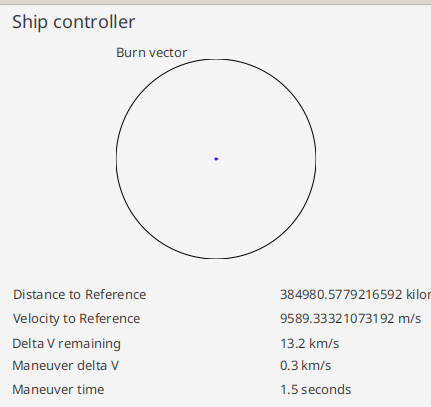
\includegraphics[width=\textwidth]{res/burn3.png}
		\caption{Maneuver: Nach 9 sec: Reduktion Maneuver delta V und Dauer}
	\end{minipage}
	\hfill
	\begin{minipage}[b]{0.45\textwidth}
		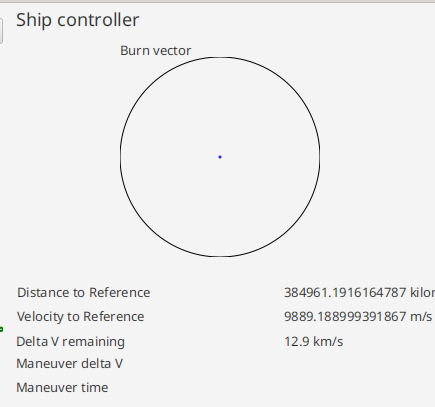
\includegraphics[width=\textwidth]{res/burn4.png}
		\caption{Maneuver: Nach 11 sec: Ende des Maneuvers, Maneuver-Linie und Informationen entfernt}
	\end{minipage}
\end{figure}

\subsection{Speichern des Simulationszustandes}
Klicken sie auf den Save-Button. 
Die Mission ist nun gespeichert. 
Eine Informationspopup erscheint zur Bestätigung.

\begin{figure}[H]
	\centering
	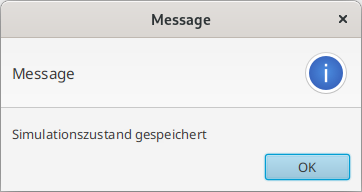
\includegraphics[width=0.45\textwidth]{res/simsaved.png}
	\caption{Simulation Speicherbestätigung}
\end{figure}
 